\documentclass[11pt]{sdm_internship}
\usepackage[british]{babel}

\usepackage{graphicx}
\graphicspath{{../img/}}

\usepackage{caption}
\usepackage{subcaption}
\usepackage{cleveref}
\usepackage{comment}
\usepackage{wrapfig}
\usepackage{amsfonts}
\usepackage{textcomp}

\pagestyle{plain}

\usepackage{hyperref}
\usepackage{url} \urlstyle{sf}
\newcommand{\email}[1]{\href{mailto:#1}{#1}}

\usepackage{xspace}

\usepackage[dvipsnames]{xcolor}
\newcommand{\addref}[1]{\colorbox{TealBlue!100}{\textcolor{white}{\textbf{$[$\ifx&#1&\ \else#1\fi$]$}}}}
\newcommand{\todo}[1]{\colorbox{Red!75}{\textcolor{white}{\textbf{TODO\ifx&#1&\else: #1\fi}}}}
\newcommand{\done}{\colorbox{YellowGreen!100}{\textcolor{white}{\textbf{DONE}}}}
\newcommand{\review}{\colorbox{YellowOrange!100}{\textcolor{white}{\textbf{REVIEW}}}}

\newcommand{\dspot}{DSpot\xspace}

\usepackage[newfloat]{minted}
% \usepackage{inconsolata}
% \setmonofont{Inconsolatazi4}

\usepackage{ragged2e}

\usepackage{amsthm}
\theoremstyle{definition}
\newtheorem{definition}{Definition}[section]

\title{Adapting Amplified Unit Tests for Human Comprehension}

\author{Simon \textsc{Bihel}}
\supervisorOne{Benoit \textsc{Baudry}}
\supervisorTwo{~}
\team{KTH Royal Institute of Technology}
\school{ens-Rennes}

\domain{Domain: Software Engineering --- Artificial Intelligence}

\abstract{%
  \justify{%
    \todo{}
  }
}


% Ought to be between 30 and 50 pages

\begin{document}
\maketitle

% ================================================================================
\section*{Introduction}%
\label{sec:intro}%
\addcontentsline{toc}{section}{\nameref{sec:intro}}
\todo{}


% ================================================================================
\section{Background}%
\label{sec:background}
In this section, we present the landscape this thesis fits into.
We define testing (Section~\ref{ssec:software_testing}) as well as go over its use in the industry.
In particular, to understand the needs of practitioners, we present how they assess the quality of their code (Sections~\ref{ssec:elementary_metrics} and~\ref{ssec:mutation_testing}) and what it takes for a new tool to be incorporated in their workflow (Sections~\ref{ssec:need_easy} and~\ref{ssec:cognitive_support_unit_test}).

% --------------------------------------------------------------------------------
\subsection{Software Testing}%
\label{ssec:software_testing}
In this section we give a definition for the test activities and their actors, the different abstraction levels of tests, and our precise object of study, unit tests.

\todo{Why are we testing software and how do we do it}

\todo{Say that the formal definitions aren't totally necessary}

% - - - - - - - - - - - - - - - - - - - - - - - - - - - - - - - - - - - - - - - -
\subsubsection{Test Activities}%
\label{sssec:test_activities}
\todo{the text is too close to the oracle survey}

Testing is about verifying that a system, for a given scenario, follows a certain behaviour that was previously defined.
The \emph{System-Under-Test} (SUT), in our domain a software system, has a set of components $C$.
A scenario is sequence of stimuli that target a subset of $C$, and trigger responses: (i) feedbacks from the SUT\@; and (ii) changes in the state of its components.
From~\cite{barr2015oracle}, we have the following definition for to combination of stimuli and responses:

\begin{definition}[Test Activities]
  For the SUT $p$, $S$ is the set of stimuli that trigger or constrain $p$'s computation and $R$ is the set of observable responses to a stimulus of $p$.
  $S$ and $R$ are disjoint.
  Test activities form the set $A = S\uplus{}R$.
  The disjoint union is used to label the elements of $A$.
\end{definition}

\begin{wrapfigure}[15]{R}{22em}
  \centering
  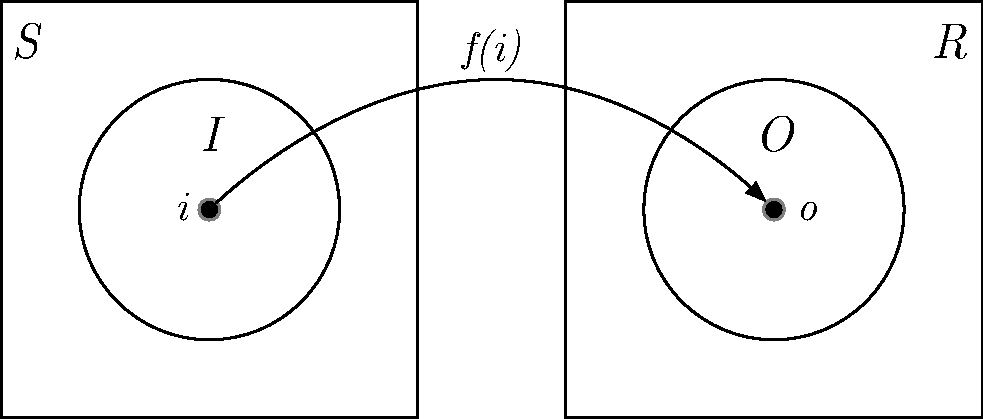
\includegraphics[width=22em]{stim_and_obs}
  \caption{Stimuli and observations: $S$ is anything that can change the observable behaviour of the SUT $f$; $R$ is anything that can be observed about the system's behaviour; $I$ includes $f$'s explicit inputs; $O$ is its explicit outputs; everything not in $S \cup R$ neither affects nor is affected by $f$.}%
  \label{fig:test_activity}
\end{wrapfigure}

The use of the terms ``stimulus'' and ``observations'' fits various test scenarios, functional and non-functional.
As depicted in \figurename~\ref{fig:test_activity}, a stimulus can be either an explicit \emph{input} from the tester, or an environmental factor that can affect the SUT\@.
Stimuli include, among others, the platform, the language version, the resources available, interaction with an interface, etc.
Observations encompass anything that can be discerned and measured like the content of a database, the visual responses on a computer screen, the time passed during the execution, etc.

Testing is about stimulation and observation so we talk about \emph{test activity sequences} that are comprised of at least one stimulus and one observation.
But testing is also about verifying that the observed responses, the behaviour, match to ones that were previously defined.
This checking part is done by another actor:

\begin{definition}[Test Oracle]
  A test oracle $D : T_A \mapsto \mathbb{B}$ is a partial function from a test activity sequence to true or false.
\end{definition}

An oracle can be defined using different methods: a set of specifications an expected value for a variable after the execution of a particular test activity sequence, the expectation of a lack of crash, etc.

A test oracle is a partial function because it can leave certain elements of the SUT's behaviour unspecified.
This part of uncertainty is fundamental in the real world because systems have grown to be so complex that humans cannot anticipate all the reactions of the SUT in all environments.
It is useful nonetheless to have a name for a theoretical oracle that would have an answer for every possible question:

\begin{definition}[Ground Truth]
  The ground truth oracle, $G$, is a total test oracle that always gives an answer.
\end{definition}

This allows us to define two properties for all oracles:

\begin{definition}[Soundness]
  The test oracle $D$ is sound for test activity $a$ iff $D(a) \rightarrow G(a)$
\end{definition}
\begin{definition}[Completeness]
  The test oracle $D$ is complete for test activity $a$ iff $G(a) \rightarrow D(a)$
\end{definition}

A test oracle cannot, in general, be complete as it would require handling every possible test activity sequence.
It is not rare for an oracle to be unsound as humans can make errors writting specifications.

In practice, following pattern designs of modularity, the act of testing is composed of multiple test activity sequences that target specific elements of the SUT's behaviour:

\begin{definition}[Test Case]
  A test case $T_C$ is a test activities sequence that contains at least one stimulus and one observation with a test oracle that verifies each observation.
\end{definition}
\begin{definition}[Test Suite]
  A test suite is a collection of tests cases.
\end{definition}

Another concept that we will use when talking about software evolution is regression testing~\cite{yoo2012regression}:

\begin{definition}[Regression Testing]
  Regression testing is performed between two different versions of the SUT in order to provide confidence that newly introduced features do not interfere with the existing features.
\end{definition}

It is a way to avoid having a human write formal specification but the problem remains of trying every possible scenario and observing any useful response.

\todo{give some clues to each concept to tell why it is a field of research?}

% - - - - - - - - - - - - - - - - - - - - - - - - - - - - - - - - - - - - - - - -
\subsubsection{Levels of Testing}%
\label{sssec:levels_testing}
\begin{wrapfigure}{L}{25em}
  \centering
  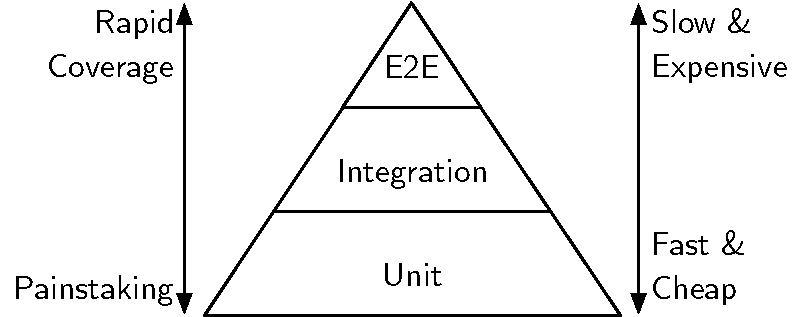
\includegraphics[width=25em]{test_pyramid}
  \caption{A view of the test pyramid.}%
  \label{fig:test_pyramid}
\end{wrapfigure}

In the case of software testing, the SUT can be different elements of a program, i.e.\ it can belong to different levels of abstraction.
One can decide to test a whole program, by manually giving inputs and verifying that the output is correct.
Or one could test individual functions, having a more control over the behaviour of each elements.

These levels of test abstraction can be visualised with a test pyramid, as shown in \figurename~\ref{fig:test_pyramid}.
Tests are generally separated into three distinct categories.
The top category is for the End-to-End tests, which means testing the program as a whole.
It can mean interacting with the UI and evaluating the visual responses.
Whilst it allows for directly evaluating the well behaviour of the program, each test is costly in time and resources because the whole program has to be run.
Not only will each component be run, whether or not it requires testing, but time will also be spent on call to libraries that are already tested.
At the other end of the test spectrum are the unit tests.
The goal is to test each and every component of the program (e.g.\ every function), as an individual and isolated from the rest of the program.
Running a single component is faster than running the whole program, but require much more work from the person writing tests, as every component needs its set of tests.
In between the two testing practices are the integration tests, which aim at ensuring the well collaboration of components, like verifying that gears rotate in the right way.
Examples of integration tests include API testing, or simply the fact of calling a function using the result from another function call.
This last example gives an intuition on how fuzzy the distinctions between all kinds of tests are, with definitions often relying on personal opinions\footnote{\url{https://testing.googleblog.com/2009/07/software-testing-categorization.html}}.
More details about the loose definition of unit tests are given Section~\ref{sssec:unit_testing}.

\todo{why we use a pyramid}
Practitioners often recommend putting an emphasis on unit test, with a distribution of 70\% unit tests, 20\% integration tests, and 10\% end-to-end tests for example\footnote{\url{https://testing.googleblog.com/2015/04/just-say-no-to-more-end-to-end-tests.html}}.

\todo{how tests are automated}

% - - - - - - - - - - - - - - - - - - - - - - - - - - - - - - - - - - - - - - - -
\subsubsection{Unit Testing}%
\label{sssec:unit_testing}

A unit test is test for a precise component of the SUT, but defining the level of granularity is not trivial, even for experienced programmers\footnote{\url{https://martinfowler.com/bliki/TestPyramid.html}}\footnote{\url{https://martinfowler.com/bliki/UnitTest.html}}~\cite{runeson2006survey}.
\todo{}

\begin{listing}[H]
  \centering
  \begin{minted}[linenos,frame=topline,breaklines,highlightlines={2,4,6},highlightcolor=YellowOrange!20]{java}
testIterationOrder() {
  TreeList tl = new TreeList(10);
  for (int i = 0; i < 10; i++) {
    tl.add(i);
  }
  ListIterator it = tl.listIterator();
  \end{minted}
  \begin{minted}[linenos,frame=bottomline,breaklines,firstnumber=last,highlightlines={10},highlightcolor=YellowGreen!20]{java}
  int i = 0;
  while (it.hasNext()) {
    Integer val = it.next();
    assertEquals(i++, val.intValue());
  }
}
  \end{minted}
  \caption{Example of an object-oriented unit test (taken from the Apache Commons Collections, in the class TreeListTest, line 270): it consists of test inputs (lines 2--6) that manipulate the SUT\@; and assertions (line number 10).\todo{what about lines 8 \& 9}}%
\label{lst:test_example}
\end{listing}

An example of unit test is given in \listingname~\ref{lst:test_example}.

\todo{why we sometimes speak about test methods}

\todo{can we link blog post from google and martin fowler to say that it's a difficult engineering problem}

\todo{evoke `software artifact'}

\todo{problems with OO, private methods, composition design patterns~\cite{wolfgang1994design}}

\todo{it's a program (and thus it carries pros and cons on comprehension and ease of use) (and it's a internal DSL~\cite{fowler2010domain})}

\todo{having small focused tests also reduce the likelihood of having a flaky test\footnote{\url{https://testing.googleblog.com/2017/04/where-do-our-flaky-tests-come-from.html}}}

\todo{dependencies\footnote{\url{https://martinfowler.com/bliki/UnitTest.html}}}

% --------------------------------------------------------------------------------
\subsection{Elementary Metrics}%
\label{ssec:elementary_metrics}
Metrics have been developed to help developers automatically assess the quality of their code.
Each metric measures one specific characteristic, such as the need for refactoring, the size of the program, or --- and we are particularly interested in this one --- the likelihood of bugs.

\todo{give examples for other metrics?}

The most basic metrics to measure how thoroughly tested a system is, are coverage based metrics.
For example, during the test suite execution, one can keep track of all statements that were executed.
At the end, you have a percentage of executed statements for the total number of statements.
Instead of statements, one can also keep track of control flow branches explored.

It is generally acknowledged that a system with high coverage means that the system is less likely to have bugs ---  but it is not foolproof.

\todo{What are their limits}
\begin{itemize}
  \item doesn't mean corner cases are avoided
  \item can't have 100\% branch coverage so it's confusing
\end{itemize}

\todo{\footnote{\url{https://testing.googleblog.com/2009/09/7th-plague-and-beyond.html}}Metrics change behavior and once a tester knows how the measurement works, they test to make themselves look good or say what they want it to say ignoring other more important factors. The metric becomes the goal instead of measuring progress.}

% --------------------------------------------------------------------------------
\subsection{Mutation Testing}%
\label{ssec:mutation_testing}
\begin{wrapfigure}[23]{L}{9em}
  \centering
  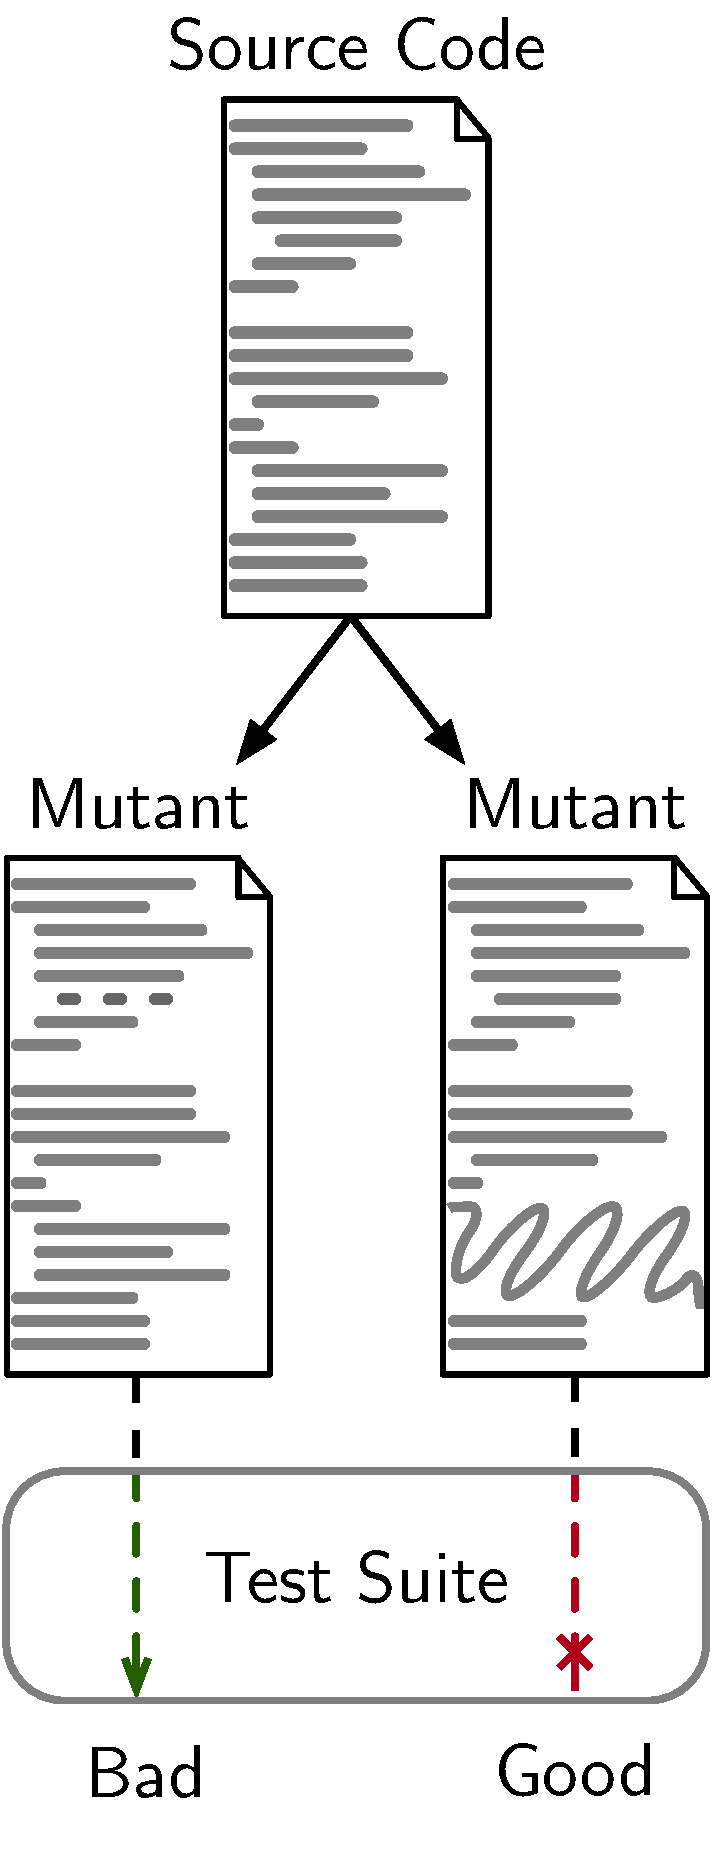
\includegraphics[width=9em]{mutation_testing_report}
  \caption{Mutation testing process.}%
\label{fig:mutation_testing}
\end{wrapfigure}
% Introduction
Mutation testing is a method used to assess the quality of a test suite, giving it a grade called \textit{mutation score}.
The idea is to insert bugs in the software and see if these faulty versions still pass the tests or not.
We call the derived versions \textit{mutants}, hence the name mutation testing.
When a mutant goes through the test suite without making a single test fail, it is considered \emph{live}, and the opposite case it is considered \emph{dead}.
The global process is depicted in~\figurename~\ref{fig:spaces}.
The main appeal is that, a test suite with a good mutation score, in addition to ensure the well behaviour of the SUT in useful scenarios, it can detect bad behaviours --- which is particularly useful for regression testing.
\todo{rework that sentence}
There is a correlation between mutation score and coverage score as test suites with high mutation score tend to have good coverage~\cite{assylbekov2013investigating}.
It has been found that correlations between mutation scores and real fault detection are weak~\cite{papadakis2018mutation}.

\todo{a mutation covered line is stronger than a regular covered line}

\addref{fundational papers}

% Mutators
Mutants are obtained by applying \emph{mutators} on the original version.
These operators can be varied: change a condition (e.g.\ substituting $\leq$ with $>$), delete the body of a method \addref{descartes}, etc.
Most of the time, we generate 1-\emph{order} mutants, that means that a mutant is the result of a mutator applied once.
A mutator will usually generate several mutants.
For example, a mutator that replaces a \texttt{while} statement into a \texttt{do-while} statement will generate a mutant for each \texttt{while} in the artifact.
In the case of $k$-order mutants, which can be thought of as the result of $k$ succesive 1-order mutants\cite{wah2000theoretical}, the number of derived programs starts to blow up.

% Difficulties
Mutation testing suffers from drawbacks that have limited its use outside of the research world even though it has been an active research domain for many years~\cite{jia2011analysis}.
The first obvious flaw is that it is slow.
For compiled languages, all mutants have to be compiled, and that process often takes a lot of time for large programs.
Then the whole test suite has to be executed for each mutant, which again is a long process.
However, given certain trade-offs in terms of quality of the mutation analysis process (e.g.\ not generating all possible mutants), the computational complexity can be dodged~\cite{offutt1993experimental,movzucha2016mutation}.
Optimized techniques for regression testing also exist~\cite{yoo2012regression}, including minimisation, selection and prioritisation, which can reduce the execution time of the test suite.
The mutant generation is also full of traps.
The major pitfall that cannot be avoided is the equivalent mutant problem.
Some mutants, although they have a different program than the original, have the same semantics.
Which means that they will always pass the test suite and will not bring any insight on the SUT\@.
The generation of mutants that are simply syntactically valid is also a non-trivial problem that requires pattern replacement instead of simple text replacement~\cite{simao2009transformational}.

Another difficulty for mutation testing to take on in the industry is the lack of understanding by practitioners.\todo{rework that sentence}
The process of mutation and elimination can be confusing.
But also, when a mutant is live, it is not always clear what actions should be taken in order to kill it.
\todo{maybe add more}

% Pitest
PIT\footnote{\url{http://pitest.org/}}~\cite{coles2016pit} is a mutation testing tool for Java.

\todo{what is great about it}

\todo{maybe quick comparison with other tools}

\todo{it is deterministic}

% --------------------------------------------------------------------------------
% \subsection{Software Diversification}%
% \label{ssec:software_diversification}
% \todo{}

% --------------------------------------------------------------------------------
\subsection{The Need for Easy-to-use Tools}%
\label{ssec:need_easy}
\todo{easy to understand}
\todo{useful for surveys}
\cite{delahaye2015selecting}

\todo{tests are written by regular developers, even though there are engineers specialised in testing\footnote{\url{https://testing.googleblog.com/2016/03/from-qa-to-engineering-productivity.html}}}
\todo{hard to move the industry forward}
\todo{we share similar experience with static analysis tool researchers}
\todo{avoid false positives, angry developers, must feel they benefit from the tool, enjoy using it~\cite{bessey2010few,sadowski2018lessons}}
\todo{\emph{effective false positives}~\cite{sadowski2015tricorder}}

% --------------------------------------------------------------------------------
\subsection{Cognitive Support Tool Development}%
\label{ssec:cognitive_support}
\todo{}
\cite{oviatt2006human}
\cite{stol2016grounded}

\todo{case studies~\cite{flyvbjerg2006five}}


% ================================================================================
\section{Test Suite Amplification}%
\label{sec:test_suite_amplification}
In this Section, we provide more context for this thesis' contribution.
\todo{}

% --------------------------------------------------------------------------------
\subsection{Genetic Improvement}%
\label{ssec:genetic_improvement}
\todo{}
\cite{petke2017genetic}
\addref{fundational papers}

\todo{part of SBSE~\cite{mcminn2011search}}

\addref{the surprising creativity of digital evolution?}

% --------------------------------------------------------------------------------
\subsection{Test Amplification}%
\label{ssec:test_amplification}
\todo{}
\cite{danglot2017emerging}\addref{A Systematic Literature Review on Test Amplification}
\cite{yoo2012test,xuan2016b,xuan2015dynamic,baudry2005automatic}

\todo{avoid overfitting}

\todo{often only partial coverage\footnote{\url{https://testing.googleblog.com/2014/07/measuring-coverage-at-google.html}}}

% --------------------------------------------------------------------------------
\subsection{\dspot{}}%
\label{ssec:dspot}
\begin{figure}
  \centering
  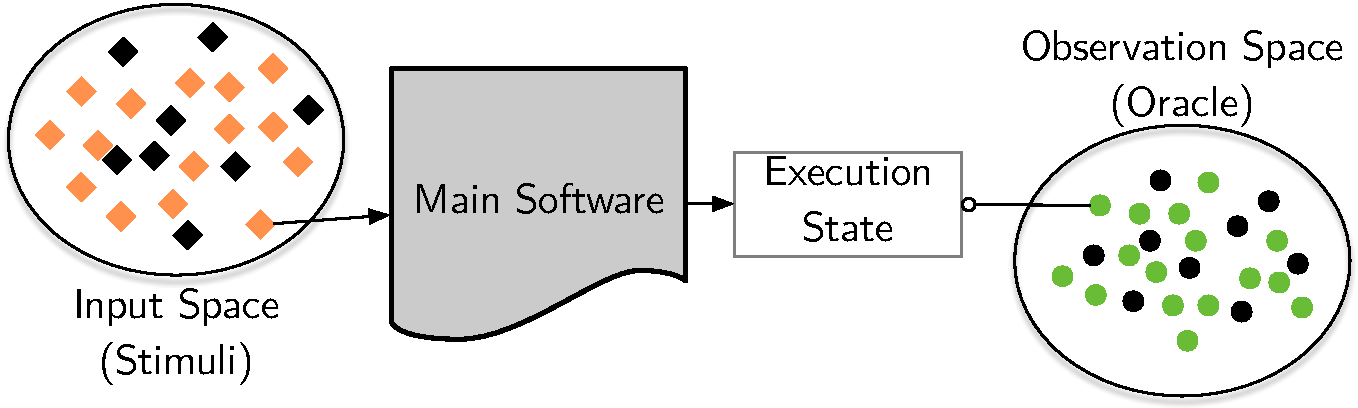
\includegraphics[width=35em]{spaces_report}
  \caption{On the left, the testing input space is composed by specified input points (orange diamonds) and unspecified input points (black diamonds). On the right, the observation space over a given program state depicts the assertions of tests. The green circles are values that are already asserted in the existing test suite, the newly added assertions are shown as black circles.}%
\label{fig:spaces}
\end{figure}
\todo{}
\footnote{\url{https://github.com/STAMP-project/dspot}}\addref{Genetic-Improvement based Unit Test Amplification for Java}\cite{baudry2015automatic,baudry2014tailored,baudry2015dspot}

\cite{pawlak2016spoon}

\todo{only produces 1-order mutants}\todo{that's confusing to say mutants for amplified tests}

\todo{finding bugs is easy~\cite{hovemeyer2004finding}}


% ================================================================================
\section{Problem Statement}%
\label{sec:problem_statement}
This thesis aim at helping developers understand amplified tests.
There are two sides for this problem: supporting the developer understand the test (Section~\ref{ssec:need_doc}) and cleaning the tests from the noise injected during the amplification process (Section~\ref{ssec:random_noise}).

\todo{understanding the test is essential~\cite{bessey2010few,sadowski2018lessons}}

% --------------------------------------------------------------------------------
\subsection{The Need for Unit Test Cases Documentation}%
\label{ssec:need_doc}
\todo{}
Several works have highlighted the need for test documentation~\cite{prado2015wap,prado2016advances,prado2018towards,li2016automatically,daka2014survey,panichella2016impact}.

\todo{tests are complex}

\todo{lack of why information}

\todo{the code the test interacts with; what the code does; what is expected}

\todo{programmers like short textual description}

\todo{explain what li2016automatically has done}

\todo{talk about the field of software maintenance~\cite{swanson1976dimensions}}

\todo{lack of work on generating human friendly descriptions for mutation testing}

% --------------------------------------------------------------------------------
\subsection{The Generated Random Noise}%
\label{ssec:random_noise}
\todo{}


% ================================================================================
\section{Related Works}%
\label{sec:related_works}
\todo{}

% --------------------------------------------------------------------------------
\subsection{Automatic Test Case Documentation}%
\label{ssec:test_doc}
\todo{}

\todo{paraphrasing the code; lack of why information}

\todo{stereotypes are for general purpose code}

\cite{neubig2016survey,nazar2016summarizing,li2016automatically,li2018automatically,kamimura2013towards,ghafari2015automatically}

\todo{there are also works on documenting code changes (i.e.\ commits)}
\cite{cortes2014automatically,linares2015changescribe,dragan2011using,jiang2017towards,jiang2017automatically,shen2016automatic,buse2010automatically}

\todo{works on describing code written by humans~\cite{wang2018comment,dragan2006reverse,dragan2011emergent,moreno2012jstereocode,buse2008automatic,sridhara2010towards,herbert2016swummary,mcburney2016automatic,sridhara2011automatically,moreno2013automatic} (e.g.\ mining comments, method and class stereotypes (too general purpose), summary, simple (syntactic) context, nl paraphrasing)}

\todo{Automatic summarization of natural language documents has been attempted by researchers for more than half a century~\cite{jones2007automatic}}

% --------------------------------------------------------------------------------
\subsection{Cognitive Support for Unit Testing Review}%
\label{ssec:cognitive_support_unit_test}
\todo{}

% --------------------------------------------------------------------------------
% \subsection{Source Code Change Documentation}%
% \label{ssec:commit_generation}
% \todo{}


% ================================================================================
\section{Contribution}%
\label{sec:contribution}
\todo{}

% --------------------------------------------------------------------------------
\subsection{Identifying Amplifications}%
\label{ssec:retrieve_amplifications}
\todo{}

% --------------------------------------------------------------------------------
\subsection{Minimisation}%
\label{ssec:minimisation}
\todo{}
\todo{put slicing before?}

\todo{removing useless assertions}

\todo{cannot use general purpose techniques\cite{leitner2007efficient,zeller1999yesterday} because we want the original part intact?}

% --------------------------------------------------------------------------------
\subsection{Replace or Keep}%
\label{ssec:replace_keep}
\todo{}

% --------------------------------------------------------------------------------
\subsection{Focus}%
\label{ssec:focus}
\todo{}
\cite{liu2006approach}

% --------------------------------------------------------------------------------
\subsection{Slicing}%
\label{ssec:slicing}
\todo{}
\cite{dolby2015tj}\footnote{\url{http://wala.sourceforge.net/}}

% --------------------------------------------------------------------------------
\subsection{Natural Language Description}%
\label{ssec:nl_description}
\todo{}

\todo{Focus on mutation testing}

\todo{avoid talking about mutants}
\todo{How to describe a mutant}

\todo{SWUM~\cite{hill2010integrating}}
\cite{alali2008s,hattori2008nature,letovsky1987cognitive}

List of possible information:
\begin{itemize}
  \item control flow branches
  \item name of mutant
  \item code under test~\cite{qusef2011scotch}
  \item traceability link
  \item label/stereotype
\end{itemize}

\todo{on the usefulness of nlg}

% --------------------------------------------------------------------------------
\subsection{Ranking}%
\label{ssec:ranking}
\todo{}


% ================================================================================
\section{Evaluation}%
\label{sec:eval}
\todo{}

% --------------------------------------------------------------------------------
\subsection{Threat to Validity}%
\label{ssec:threat_to_validity}
\todo{}

\todo{DSpot is not yet established and recognized in the community. It's is difficult to have input data (valid amplified tests)}


% ================================================================================
\section*{Conclusion}%
\label{sec:conclu}%
\addcontentsline{toc}{section}{\nameref{sec:conclu}}
\todo{}


% ================================================================================
\section*{Acknowledgments}%
\label{sec:ack}%
\addcontentsline{toc}{section}{\nameref{sec:ack}}
Thanks to Benoit Baudry and Martin Monperrus for their guidance.
Thanks to Benjamin Danglot for his collaboration and all his work on \dspot.
Thanks to Zimin Chen, Nicolas Harrand, He Ye and Long Zhang for making daily life enjoyable.
This internship was supported by the Fondation Rennes 1 and its patrons.
Many thanks to KTH for hosting me.


% ================================================================================
\bibliographystyle{ieeetr}%
\bibliography{../bibl}
\addcontentsline{toc}{section}{References}

\end{document}
